%% =====================================================================
%%  Conflict-Preserving Reversal
%%  Journal-submission manuscript (portable amsart source).
%%
%%  TARGET VENUE (default): Journal of Automated Reasoning (Springer).
%%  This file is deliberately venue-neutral and compiles with a plain
%%  `pdflatex` pass (manual bibliography, no bibtex). To submit, drop the
%%  body into the target journal's class (e.g. Springer Nature sn-jnl for
%%  JAR/Constraints; AAAI/IJCAI styles for a conference) and convert the
%%  References block to that venue's .bst style.
%%
%%  >>> BEFORE SUBMISSION: fill every placeholder marked  <<...>>  below,
%%      especially the author identity block and the artifact DOI.
%% =====================================================================
\documentclass[11pt,reqno]{amsart}

\usepackage[T1]{fontenc}
\usepackage{lmodern}
\usepackage{amsmath,amssymb,amsthm,mathtools}
\usepackage{xcolor}
\usepackage{booktabs}
\usepackage{array}
\usepackage{makecell}
\usepackage{tikz}
\usetikzlibrary{arrows.meta,positioning,calc,decorations.pathreplacing}
\usepackage[margin=1in]{geometry}
\usepackage{microtype}
\usepackage[colorlinks=true,linkcolor=blue!55!black,citecolor=blue!55!black,urlcolor=blue!55!black]{hyperref}

% ---- theorem environments (numbered independently per type, matching the
%      original manuscript: Theorem 1, Theorem 2, Lemma 1, ... ) ----------
\theoremstyle{plain}
\newtheorem{theorem}{Theorem}
\newtheorem{proposition}{Proposition}
\newtheorem{lemma}{Lemma}
\newtheorem{corollary}{Corollary}
\theoremstyle{definition}
\newtheorem{definition}{Definition}
\newtheorem{example}{Example}

% ---- operators and shorthands ----------------------------------------
\DeclareMathOperator{\Exp}{Exp}
\DeclareMathOperator{\Rev}{Rev}
\DeclareMathOperator{\Conj}{Conj}
\newcommand{\Mstar}{M^{*}}
\newcommand{\sd}{\mathbin{\triangle}}        % symmetric difference
\newcommand{\PRUNE}{\textsc{Prune}}
\newcommand{\FWD}{\textsc{Fwd}}
% a visible placeholder marker for pre-submission fields
\newcommand{\placeholder}[1]{{\normalfont\sffamily\color{red!60!black}$\langle\!\langle$#1$\rangle\!\rangle$}}

% ---- a dependency-free algorithm box ---------------------------------
\newcounter{algline}
\newenvironment{algobox}[1]
  {\par\medskip\noindent\begin{tabular}{@{}p{\dimexpr\linewidth-2\tabcolsep}@{}}
   \toprule \textbf{Algorithm 1}\quad #1\\ \midrule}
  {\\ \bottomrule\end{tabular}\par\medskip}

% ---- hanging-indent reference list (no bibtex needed) ----------------
\newenvironment{references}
  {\section*{References}\small\setlength{\parindent}{0pt}%
   \everypar{\hangindent=1.6em\hangafter=1}\setlength{\parskip}{3pt}}
  {\par}

\begin{document}

\title[Conflict-Preserving Reversal]{Conflict-Preserving Reversal:\\
Exact Rollback and Order-Determined Minimal Conflicts\\ in Propositional Expansions}

\author{Rinzl3r}
\address{Independent researcher}
\email{\placeholder{contact email -- required before submission}}
\thanks{\emph{Author identity to be completed before submission.} Most journals
require a legal name, an affiliation (``Independent Scholar'' is acceptable), a
corresponding-author email, and an ORCID iD\,(\placeholder{0000-0000-0000-0000}).
``Rinzl3r'' is a pseudonymous handle and should be replaced or formally
disclosed to the editor.}

\date{Revised November 2026}

\subjclass[2020]{03B05, 68R07, 68T27, 68N30}
\keywords{propositional logic; incremental SAT; minimal unsatisfiable subsets;
preferred conflicts; assumption retraction; delta debugging; fault localization;
model-based diagnosis}

\begin{abstract}
Exploratory proof development, incremental SAT solving, and automated debugging
share an operational pattern: a satisfiable base formula $S$ is strengthened by a
sequence of retractable assumptions $c_1,\dots,c_n$, each discharged to a
satisfiability oracle and later retracted. We isolate two failure modes of this
pattern. \emph{Provenance loss} occurs when contexts are stored by content, so
that retracting an assumption silently deletes a duplicated background conjunct
and weakens $S$. \emph{Diagnostic misattribution} occurs because the transition
assumption at which a prefix first becomes unsatisfiable belongs to every
conflict in that prefix yet rarely explains it. We prove that a positional record
makes rollback exact, and we establish a \emph{Conflict-Preserving Reversal
Theorem}: reversing the expansion while retaining exactly those assumptions whose
removal would restore satisfiability performs exactly $n$ oracle calls and returns
the colexicographically least minimal unsatisfiable subset, which coincides with
the preferred conflict of preference-based diagnosis. The result holds for every
monotone predicate, giving a common foundation for change-set minimization in
delta debugging, formula-based fault localization, consistency-based diagnosis,
and type-error localization. We further show that the scan direction selects, at
identical cost, between the chronologically earliest and the most recent
explanation, and we report exhaustive and randomized experiments that quantify
both failure modes.
\end{abstract}

\maketitle

\noindent\textbf{ACM CCS 2012.}\quad
Theory of computation $\rightarrow$ Logic $\rightarrow$ Automated reasoning;\;
Computing methodologies $\rightarrow$ Knowledge representation and reasoning;\;
Software and its engineering $\rightarrow$ Software testing and debugging.

\medskip

% =====================================================================
\section{Problem Statement: Two Failure Modes in Conjectural Expansion}
% =====================================================================
Many reasoning workflows maintain a mutable context under a stack discipline. A
satisfiable base formula $S$ (hard constraints, a background baseline, a passing
baseline) is extended by an ordered sequence of retractable assumptions
$c_1,\dots,c_n$ (conjectures, soft constraints, candidate changes); each extension
is discharged to a SAT or SMT oracle; and the assumptions are subsequently
retracted. Incremental SAT interfaces (Hooker, 1993; E\'en \& S\"orensson, 2003,
2004), SMT-LIB assertion stacks (Barrett et al., 2026), and interactive proof
development and automated debugging (Zeller, 1999; Jose \& Majumdar, 2011) are all
instances of this pattern. This paper determines what metadata the context must
carry for retraction to be exact, and what an unsatisfiable oracle answer licenses
one to conclude about the cause of the failure.

\paragraph{Failure mode 1: provenance loss under content-based retraction.}
If the active context is represented extensionally---as a set of conjuncts, a
deduplicated clause database, or a deductively closed theory (Alchourr\'on et al.,
1985)---the representation forgets \emph{which occurrence} of a formula an
assumption contributed. Retracting $c_k$ then also deletes any background conjunct
syntactically identical to a conjunct of $c_k$, so subsequent oracle calls are
posed against a strictly weaker background and may return spurious SAT verdicts.

\paragraph{Failure mode 2: diagnostic misattribution at the first inconsistent
prefix.} If the prefix context first becomes unsatisfiable upon adjoining $c_j$,
it is tempting to report $c_j$ as the cause. In general $c_j$ is satisfiable
together with $S$; the inconsistency arises from its interaction with a subset of
$c_1,\dots,c_{j-1}$. The phenomenon is familiar from type inference, where
compilers report the location at which constraint solving failed rather than the
actual error source (Pavlinovic et al., 2014). Conversely, the standard forward
deletion scan may return an explanation that contains assumptions added after
step $j$.

\paragraph{Contributions.}
\begin{enumerate}
\item Proposition~1 characterizes exact retraction: for formula strings the pair
$(F_n,n)$ is a lossless encoding of $(S,c)$, whereas extensional stores retract
exactly if and only if the retracted conjuncts are disjoint from the remainder.
Corollary~1 shows that selector (activation) literals restore this disjointness.
\item Theorem~1 (Conflict-Preserving Reversal) proves that conditional reversal
(Algorithm~1, \PRUNE) computes, with exactly $n$ oracle calls, the
colexicographically least $S$-conflict $\Mstar$; this conflict is minimal, has the
transition index $j$ as its maximum, and coincides with Junker's (2004) preferred
conflict.
\item Theorem~2 lifts the result to arbitrary monotone predicates in the sense of
Marques-Silva et al.\ (2013), which makes it applicable to failure-inducing change
sets, trace formulas over SMT theories, and diagnosis problems.
\item Corollaries~2--4 establish order completeness over minimal conflicts, the
exact diagnostic content of the first inconsistent prefix, and a scan-direction
duality for deletion-based MUS extraction. Section~5 maps the results onto
debugging methodology, Section~6 positions them relative to existing methods, and
Section~7 reports experiments.
\end{enumerate}

% =====================================================================
\section{Formal Setup}
% =====================================================================
\begin{definition}[Language, expansion, reversal]
Let $L$ be the set of fully parenthesized propositional formulas over atoms
$p,q,r,\dots$ and the connectives $\neg,\wedge,\vee,\rightarrow$; equality of
formulas is syntactic identity, and $\vDash$ is classical consequence (Enderton,
2001; Mendelson, 2015). A \emph{trace} is a finite sequence
$c=(c_1,\dots,c_n)\in L^n$. The \emph{expansion} of $S\in L$ along $c$ is the
left-nested sequence
\begin{equation}
F_0=S,\qquad F_k=(F_{k-1}\wedge c_k)\quad(1\le k\le n),
\end{equation}
with $\Exp(S,c)=F_n$. \emph{Reversal} sets $G_n=F$ and, for $k=n,\dots,1$,
$G_{k-1}=A$ whenever $G_k=(A\wedge c_k)$; it returns $\Rev(F,c)=G_0$ if every step
is defined.
\end{definition}

\begin{lemma}[Unique readability; exact reversal]
If $(A\wedge B)$ and $(A'\wedge B')$ are identical strings, then $A=A'$ and
$B=B'$. Consequently $\Rev(\Exp(S,c),c)=S$ for every $S\in L$ and every trace $c$.
\end{lemma}
\begin{proof}
The first statement is the unique readability theorem for fully parenthesized
formulas (Enderton, 2001, Chapter~1). For the second, downward induction gives
$G_k=F_k$: if $G_k=F_k=(F_{k-1}\wedge c_k)$, unique readability forces
$G_{k-1}=F_{k-1}$.
\end{proof}

\begin{definition}[Subtraces and conflicts]
Write $[m]=\{1,\dots,m\}$ and $[0]=\varnothing$. For $I\subseteq[n]$ with elements
$i_1<\dots<i_m$, let $c|_I=(c_{i_1},\dots,c_{i_m})$ and $F^I=\Exp(S,c|_I)$, so that
$F_k=F^{[k]}$. The set $I$ is \emph{$S$-consistent} if $F^I$ is satisfiable and an
\emph{$S$-conflict} otherwise; an $S$-conflict is \emph{minimal} (an $S$-MUS) if
every proper subset is $S$-consistent. In the terminology of high-level
(group-oriented) MUS extraction, $S$ is a hard background group that is never
blamed and each $c_i$ is a retractable group (Nadel, 2010; Ryvchin \& Strichman,
2011).
\end{definition}

\begin{lemma}[Semantics and monotonicity]
\textup{(a)} A valuation satisfies $F^I$ if and only if it satisfies $S$ and every
$c_i$ with $i\in I$; hence $F^I\vDash S$, and satisfiability of $F^I$ is invariant
under permutations of the adjoined assumptions.
\textup{(b)} The family of $S$-conflicts is upward closed in $2^{[n]}$: if
$I\subseteq J$ and $I$ is an $S$-conflict, so is $J$.
\textup{(c)} An $S$-conflict $I$ is minimal if and only if $I\setminus\{i\}$ is
$S$-consistent for every $i\in I$.
\end{lemma}
\begin{proof}
(a) is induction on $|I|$ using the truth table of $\wedge$; (b) follows from (a);
in (c), every proper subset of $I$ lies inside some $I\setminus\{i\}$, and (b)
applies.
\end{proof}

\begin{definition}[Colexicographic order; preferred conflict]
For distinct $I,J\subseteq[n]$, write $I\prec J$ if $\max(I\sd J)\in J$. The
$\prec$-least $S$-conflict, when it exists, is the \emph{preferred conflict} of
$(S,c)$, denoted $\Mstar$. This is the colexicographic order on $2^{[n]}$, and it
coincides with the anti-lexicographic order used by Junker (2004) when $c_1$ is the
most preferred constraint.
\end{definition}

\begin{lemma}[Order-theoretic properties]
Let $w(I)=\sum_{i\in I}2^{\,i-1}$.
\textup{(a)} For distinct $I,J$, $I\prec J$ if and only if $w(I)<w(J)$; thus
$\prec$ is a strict total order.
\textup{(b)} If $I\subsetneq J$, then $I\prec J$.
\textup{(c)} If $F_n$ is unsatisfiable, then $\Mstar$ exists, is unique, and is a
minimal $S$-conflict.
\end{lemma}
\begin{proof}
(a) Let $m=\max(I\sd J)$. Both sets agree above $m$, and indices below $m$
contribute at most $2^{m-1}-1<2^{m-1}$, so the set containing $m$ has the larger
weight. (b) Every element of $J\setminus I$, in particular the largest, lies in
$J$. (c) $[n]$ is an $S$-conflict, so the finite family of conflicts has a unique
$\prec$-least element; each proper subset of $\Mstar$ is $\prec$-smaller by (b) and
therefore $S$-consistent.
\end{proof}

\begin{example}[Running example; configuration-debugging reading]
Let $S=((p\rightarrow r)\wedge(q\rightarrow\neg r))$ and
$c=(p,\,(p\vee q),\,q,\,r)$. Read $p$ as \emph{GPS module enabled}, $q$ as
\emph{battery-saver profile}, and $r$ as \emph{high-power radio}: $S$ encodes two
product constraints (GPS requires the high-power radio; the battery-saver profile
forbids it), and $c$ is a sequence of user requirements entered in a configuration
session, the setting in which preferred conflicts were introduced (Junker, 2004;
Felfernig et al., 2004). Then
\begin{equation}
F_4=(((((p\rightarrow r)\wedge(q\rightarrow\neg r))\wedge p)\wedge(p\vee q))\wedge q)\wedge r.
\end{equation}
The prefixes $F_0,F_1,F_2$ are satisfiable and $F_3,F_4$ are not, so $j=3$; yet the
transition requirement $q$ is $S$-consistent in isolation. There are exactly two
minimal conflicts, $\{1,3\}=\{p,q\}$ with $w=5$ and $\{3,4\}=\{q,r\}$ with $w=12$;
hence $\Mstar=\{1,3\}$.
\end{example}

\begin{figure}[t]
\centering
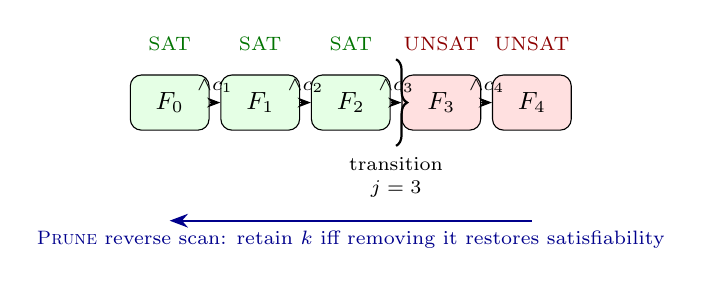
\begin{tikzpicture}[x=1.15cm,y=1cm,>=Stealth,font=\small]
  % prefix cells
  \foreach \k/\lab/\sat in {0/$F_0$/1,1/$F_1$/1,2/$F_2$/1,3/$F_3$/0,4/$F_4$/0}{
    \ifnum\sat=1
      \node[draw,rounded corners,minimum width=1cm,minimum height=.7cm,fill=green!10] (c\k) at (\k,0) {\lab};
    \else
      \node[draw,rounded corners,minimum width=1cm,minimum height=.7cm,fill=red!12] (c\k) at (\k,0) {\lab};
    \fi
  }
  \foreach \k/\n in {1/{c_1},2/{c_2},3/{c_3},4/{c_4}}{
    \pgfmathtruncatemacro\p{\k-1}
    \draw[->] (c\p) -- (c\k) node[midway,above,font=\scriptsize] {$\wedge \n$};
  }
  % transition marker
  \draw[decorate,decoration={brace,amplitude=4pt,mirror},thick]
      (2.5,-.55) -- (2.5,.55);
  \node[font=\scriptsize,align=center] at (2.5,-.95) {transition\\$j=3$};
  % satisfiability labels
  \node[font=\scriptsize,green!45!black] at (0,.75) {SAT};
  \node[font=\scriptsize,green!45!black] at (1,.75) {SAT};
  \node[font=\scriptsize,green!45!black] at (2,.75) {SAT};
  \node[font=\scriptsize,red!55!black] at (3,.75) {UNSAT};
  \node[font=\scriptsize,red!55!black] at (4,.75) {UNSAT};
  % reverse scan arrow
  \draw[->,thick,blue!55!black] (4,-1.5) -- (0,-1.5)
      node[midway,below,font=\scriptsize] {\PRUNE{} reverse scan: retain $k$ iff removing it restores satisfiability};
\end{tikzpicture}
\caption{Expansion of $S$ along the trace of Example~1. Satisfiability flips once,
at the transition index $j$; \PRUNE{} scans the trace in reverse and keeps exactly
the assumptions that the preferred conflict $\Mstar$ needs.}
\label{fig:scan}
\end{figure}

% =====================================================================
\section{Provenance and Exact Rollback}
% =====================================================================
\begin{proposition}[Positional versus extensional records]
Let $c$ have length $n$ and $F_n=\Exp(S,c)$.
\textup{(a) Depth-only recovery.} The string $F_n$ and the integer $n$ determine
$S$ and $c$: setting $G_n=F_n$ and decomposing $G_k=(G_{k-1}\wedge d_k)$ for
$k=n,\dots,1$ yields $G_0=S$ and $(d_1,\dots,d_n)=c$.
\textup{(b) Exactness criterion for extensional stores.} Let
$\Conj((B\wedge C))=\Conj(B)\cup\Conj(C)$ and $\Conj(A)=\{A\}$ for every $A$ that
is not a conjunction. If stage $k$ is stored as
$\Gamma_k=\Conj(S)\cup\Conj(c_1)\cup\dots\cup\Conj(c_k)$, then content-based
retraction $\Gamma_k\setminus\Conj(c_k)$ equals $\Gamma_{k-1}$ if and only if
$\Conj(c_k)\cap\Gamma_{k-1}=\varnothing$.
\end{proposition}
\begin{proof}
(a) Downward induction with Lemma~1: $G_k=F_k=(F_{k-1}\wedge c_k)$ forces
$G_{k-1}=F_{k-1}$ and $d_k=c_k$. (b)
$(\Gamma_{k-1}\cup\Conj(c_k))\setminus\Conj(c_k)=\Gamma_{k-1}\setminus\Conj(c_k)$,
which equals $\Gamma_{k-1}$ exactly when the two sets are disjoint.
\end{proof}

Part~(a) sharpens the impossibility of trace-free reversal. No map $R\colon L\to L$
recovers $S$ from $F_n$ alone---$S_1=p$ expanded by $(q)$ and $S_2=(p\wedge q)$
expanded by the empty trace both yield $(p\wedge q)$---but one integer of
$\lceil\log_2(n+1)\rceil$ bits suffices, because the nesting structure of the
string is itself a positional record. This is precisely the state maintained by the
level counter of an SMT-LIB assertion stack, whose \texttt{pop} discards the most
recent assertion level (Barrett et al., 2026). Part~(b) explains why explicit
provenance is indispensable for extensional stores: in a deductively closed theory,
expansion by a sentence already present is the identity, so no operation on
theories can distinguish a temporary addition from a background fact (Alchourr\'on
et al., 1985); clause databases become extensional in the same sense once duplicate
or subsumed clauses are merged, one source of the incompatibility between
preprocessing and incremental solving analysed by Nadel et al.\ (2012).

\begin{example}[Provenance loss]
Let $S'=(S\wedge p)$ with $S$ as in Example~1, so
$\Conj(S')=\{(p\rightarrow r),(q\rightarrow\neg r),p\}$. Adjoin $c_1=p$ (for
instance, because the fact reappears as an imported lemma) and retract it by
content: $\Gamma_1\setminus\{p\}=\{(p\rightarrow r),(q\rightarrow\neg r)\}$, so the
background fact $p$ has been deleted. A subsequent probe $q$ is reported
satisfiable ($q$ true, $p$ and $r$ false) although $(S'\wedge q)$ is unsatisfiable.
Positional rollback returns $\Rev((S'\wedge p),(p))=S'$ and the correct UNSAT
verdict.
\end{example}

\begin{corollary}[Selector literals restore exactness]
Store each assumption as the guarded formula $(\neg s_k\vee c_k)$, where $s_k$ is a
fresh atom occurring in no other stored formula, and activate it by solving under
the assumption literal $s_k$. Then
$\Conj((\neg s_k\vee c_k))\cap\Gamma_{k-1}=\varnothing$, so content-based deletion
of the guarded formula is exact by Proposition~1(b). Moreover $F^I$ is satisfiable
if and only if the guarded store is satisfiable under the assumptions
$\{s_i:i\in I\}\cup\{\neg s_i:i\notin I\}$.
\end{corollary}
\begin{proof}
The guarded formula is a disjunction, so its $\Conj$ is a singleton containing the
fresh atom $s_k$, which does not occur in $\Gamma_{k-1}$. Under the stated
assumptions, every guard with $i\notin I$ is satisfied by $\neg s_i$ and every
guard with $i\in I$ reduces to $c_i$; since the selectors are fresh, models of
$F^I$ extend to models of the guarded store and conversely restrict.
\end{proof}

\paragraph{Debugging application.} Corollary~1 is the formal content of the
activation-literal idiom of incremental SAT (E\'en \& S\"orensson, 2003, 2004;
Nadel \& Ryvchin, 2012) and of the selector variables with clause grouping used by
BugAssist for fault localization (Jose \& Majumdar, 2011). It shows that the idiom
is not merely an efficiency device: it is the minimal change that turns an
extensional clause store into a provenance-preserving one.

% =====================================================================
\section{Conflict-Preserving Reversal}
% =====================================================================
Plain reversal removes $c_n,c_{n-1},\dots,c_1$ unconditionally. Algorithm~1
traverses the trace in the same order but retains every assumption whose removal
would render the retained context satisfiable.

\begin{algobox}{\PRUNE$(S,c)$ --- conflict-preserving reversal}
\emph{Input:} a satisfiable base formula $S\in L$; a trace $c=(c_1,\dots,c_n)$ with
$F_n$ unsatisfiable; a SAT oracle.\\[2pt]
\emph{Output:} an index set $K\subseteq[n]$ (and the reduced expansion
$F^K=\Exp(S,c|_K)$).\\[4pt]
\begin{tabular}{@{}r@{\quad}l@{}}
1 & $K\leftarrow[n]$\\
2 & \textbf{for} $k=n,n-1,\dots,1$ \textbf{do}\\
3 & \quad \textbf{if} $F^{K\setminus\{k\}}$ is unsatisfiable \textbf{then} $K\leftarrow K\setminus\{k\}$ \quad\textit{($c_k$ is redundant for the conflict)}\\
4 & \quad \textbf{else} retain $k$ \quad\textit{($c_k$ is a transition constraint)}\\
5 & \textbf{return} $K$\\
\end{tabular}
\end{algobox}

\begin{theorem}[Conflict-Preserving Reversal]
Let $S\in L$ be satisfiable, let $c=(c_1,\dots,c_n)$ be a trace with $F_n$
unsatisfiable, let $j=\min\{k:F_k\text{ is unsatisfiable}\}$, and let $K$ be the
output of \PRUNE$(S,c)$. Then:
\begin{enumerate}
\item[\textup{(i)}] \emph{Agreement with plain reversal.} \PRUNE{} removes
$c_n,\dots,c_{j+1}$---exactly the assumptions that unconditional reversal removes
before satisfiability is restored---and retains $c_j$.
\item[\textup{(ii)}] \emph{Transition necessity.} Whenever $c_k$ is retained, every
$S$-conflict contained in the current set $K$ contains $k$; in particular $j$
belongs to every $S$-conflict $I\subseteq[j]$.
\item[\textup{(iii)}] \emph{Preference and minimality.} $K=\Mstar$; hence $K$ is a
minimal $S$-conflict and $\max K=j$.
\item[\textup{(iv)}] \emph{Oracle complexity.} \PRUNE{} performs exactly $n$ oracle
calls, and consecutive queries differ in at most two assumption literals.
\item[\textup{(v)}] \emph{Exact rollback.} Every tested formula and the output
$F^K$ are expansions of $S$ along subtraces of $c$; in particular
$\Rev(F^K,c|_K)=S$.
\end{enumerate}
\end{theorem}
\begin{proof}
Let $K_k$ denote the value of $K$ immediately before index $k$ is tested, so
$K_n=[n]$ and $K_0$ is the output.

(i) We show $K_k=[k]$ for $k=n,\dots,j$. If $K_k=[k]$ and $k>j$, line~3 tests
$[k-1]\supseteq[j]$, which is an $S$-conflict by Lemma~2(b); so $c_k$ is removed and
$K_{k-1}=[k-1]$. At $k=j$ the tested set $[j-1]$ is $S$-consistent by minimality of
$j$ (and $j\ge1$ because $S$ is satisfiable), so $c_j$ is retained.

(ii) If $c_k$ is retained, $K_k\setminus\{k\}$ is $S$-consistent; an $S$-conflict
$I\subseteq K_k$ with $k\notin I$ would lie inside $K_k\setminus\{k\}$,
contradicting Lemma~2(b). With $K_j=[j]$ from~(i) this gives the second claim.

(iii) We prove by downward induction that $K_k$ is an $S$-conflict and
$K_k=A_k\cup[k]$, where $A_k=\Mstar\cap\{k+1,\dots,n\}$. This holds for $k=n$ with
$A_n=\varnothing$. At step $k\ge1$, line~3 tests $T=A_k\cup[k-1]$. If $T$ is an
$S$-conflict, $c_k$ is removed; were $k\in\Mstar$, then $T$ and $\Mstar$ would agree
above $k$ while $k\in\Mstar\setminus T$, giving $T\prec\Mstar$ and contradicting the
leastness of $\Mstar$; hence $k\notin\Mstar$, $A_{k-1}=A_k$ and
$K_{k-1}=T=A_{k-1}\cup[k-1]$. If $T$ is $S$-consistent, $c_k$ is retained; were
$k\notin\Mstar$, then $\Mstar\subseteq T$ and $T$ would be an $S$-conflict by
Lemma~2(b); hence $k\in\Mstar$, $A_{k-1}=A_k\cup\{k\}$ and
$K_{k-1}=K_k=A_{k-1}\cup[k-1]$. In both cases $K_{k-1}$ is an $S$-conflict. At
$k=0$, $K_0=A_0=\Mstar$; minimality follows from Lemma~3(c), and $\max K=j$ from~(i).

(iv) Line~3 is executed once per $k\in[n]$. The tested sets at steps $k$ and $k-1$
are $A_k\cup[k-1]$ and $A_{k-1}\cup[k-2]$, which differ only in $k-1$ and possibly
$k$. (v) Each tested formula equals $\Exp(S,c|_T)$ for some $T\subseteq[n]$; apply
Lemma~1.
\end{proof}

By (iv), \PRUNE{} is well suited to solvers that answer queries under assumptions:
between consecutive calls at most two selector literals change polarity, so learned
clauses and heuristic state are reused across the entire scan (E\'en \&
S\"orensson, 2003; Nadel \& Ryvchin, 2012). In Example~1, \PRUNE{} drops $r$ ($F_3$
is unsatisfiable), retains $q$ ($F_2$ is satisfiable), drops $(p\vee q)$ ($\{p,q\}$
is unsatisfiable), and retains $p$ ($\{q\}$ is satisfiable), returning
$\Mstar=\{1,3\}$ after four calls.

The proof of Theorem~1 uses only two properties of satisfiability: upward closure
of conflicts (Lemma~2(b)) and consistency of the empty set. It therefore applies to
the general problem of computing a minimal set over a monotone predicate (MSMP),
which subsumes MUS, minimal correction set, and prime-implicate computation
(Marques-Silva et al., 2013).

\begin{theorem}[Monotone-predicate generalization]
Let $P\colon2^{[n]}\to\{0,1\}$ be monotone ($I\subseteq J$ and $P(I)=1$ imply
$P(J)=1$), with $P([n])=1$ and $P(\varnothing)=0$. Run Algorithm~1 with the test in
line~3 replaced by $P(K\setminus\{k\})=1$. Then the algorithm evaluates $P$ exactly
$n$ times and returns the $\prec$-least set $M_P$ with $P(M_P)=1$; $M_P$ is
$\subseteq$-minimal, and $\max M_P=\min\{k:P([k])=1\}$. Without monotonicity, the
output still satisfies $P(K)=1$, but minimality is no longer guaranteed.
\end{theorem}
\begin{proof}
Replace ``$S$-conflict'' by ``$P$-set'' in the proofs of Lemma~3 and Theorem~1;
only the upward closure of $P$-sets and $P(\varnothing)=0$ are used. Without
monotonicity, the invariant $P(K)=1$ still holds because an index is removed only
when $P(K\setminus\{k\})=1$.
\end{proof}

\begin{corollary}[Order completeness]
If $I$ is any minimal $S$-conflict and the trace is permuted so that the
assumptions indexed by $I$ precede all others, then \PRUNE{} applied to the
permuted trace returns exactly the assumptions indexed by $I$.
\end{corollary}
\begin{proof}
After the permutation $I$ occupies $[m]$, $m=|I|$. Any other conflict $J$ is not
contained in $[m]$, because a conflict properly inside the minimal conflict $[m]$
cannot exist; so $J$ has an element above $m$, $\max([m]\sd J)\in J$, and
$[m]\prec J$. Thus $[m]=\Mstar$, and Theorem~1(iii) applies.
\end{proof}

\paragraph{Debugging application.} Because $\Mstar$ minimizes reliance on late
positions, trace positions act as a \emph{blame-avoidance priority}: assumptions
that should not appear in explanations (trusted lemmas, vetted requirements) belong
late in the trace or, if they are never to be blamed, in $S$; suspect assumptions
placed early are preferentially implicated. By Corollary~2, the trace order is a
complete steering parameter for single-MUS extraction: every minimal explanation is
reachable by some order, although dedicated enumeration algorithms are more
efficient when many MUSes are required (Liffiton \& Sakallah, 2008; Liffiton et
al., 2016).

\begin{corollary}[Diagnostic content of the first inconsistent prefix]
Under the hypotheses of Theorem~1, $c_j$ belongs to $\Mstar$ and to every
$S$-conflict contained in $[j]$. Moreover, $\{j\}$ is an $S$-conflict if and only if
$\Mstar=\{j\}$; otherwise $\Mstar\setminus\{j\}$ is the trace-preferred minimal set
of earlier assumptions that, together with $S$, refutes $c_j$.
\end{corollary}
\begin{proof}
The first statement is Theorem~1(ii)--(iii). Every $S$-conflict $I$ satisfies
$\max I\ge j$, since $I\subseteq[\max I]$ makes $F_{\max I}$ unsatisfiable; hence
$w(I)\ge2^{\,j-1}=w(\{j\})$, with equality only for $I=\{j\}$. If $\Mstar\ne\{j\}$,
minimality of $\Mstar$ shows that $\Mstar\setminus\{j\}$ is $S$-consistent while
$(\Mstar\setminus\{j\})\cup\{j\}$ is not.
\end{proof}

\paragraph{Debugging application.} Halting at the first failing step identifies a
necessary transition constraint, not a cause. Corollary~3 separates an
\emph{intrinsic} fault---$c_j$ is inconsistent with $S$ on its own,
$|\Mstar|=1$---from an \emph{interaction} fault, $|\Mstar|\ge2$, in which $c_j$ is
consistent with the background but not with specific earlier assumptions. In
Example~1 the failure at the battery-saver requirement is an interaction fault with
the earlier GPS requirement.

\begin{corollary}[Scan-direction duality]
Let \FWD{} denote deletion-based extraction with the scan $k=1,\dots,n$, and let
$c^R=(c_n,\dots,c_1)$. Then \FWD{} on $c$ coincides, after index reversal, with
\PRUNE{} on $c^R$. Consequently \FWD{} performs exactly $n$ calls and returns the
$S$-conflict that is least for the reversed order $\prec^R$, where $I\prec^R J$ if
$\min(I\sd J)\in J$; this conflict is minimal, and its minimum is
$j^R=\max\{k:\{k,\dots,n\}\text{ is an }S\text{-conflict}\}$. \FWD{} and \PRUNE{}
return the same conflict if and only if the $\prec$-least and $\prec^R$-least
conflicts coincide---in particular whenever the minimal $S$-conflict is unique.
\end{corollary}
\begin{proof}
\FWD{} tests position $k$ of $c$ when \PRUNE{} tests position $n+1-k$ of $c^R$, and
both test the same sets of formulas; satisfiability is order-invariant by
Lemma~2(a). Transporting Definition~3 along $i\mapsto n+1-i$ turns $\prec$ into
$\prec^R$, and transporting $j$ for $c^R$ (the shortest unsatisfiable prefix of
$c^R$) yields the longest unsatisfiable suffix of $c$. The remaining claims follow
from Theorem~1.
\end{proof}

\paragraph{Debugging application.} The output of deletion-based MUS extraction
(Belov et al., 2012) depends on the scan order, and Corollary~4 makes the
dependence exact. At identical cost, the reverse scan yields the chronologically
earliest explanation, anchored at the step where failure became inevitable, while
the forward scan yields the most recent explanation, the natural choice under the
triage heuristic that recent changes are the likeliest culprits. In Example~1,
\FWD{} returns $\{q,r\}$, which uses the radio requirement $r$ although the session
was already inconsistent before $r$ was entered. The scan direction should
therefore be chosen as an explicit triage policy rather than left as an
implementation detail.

% =====================================================================
\section{Applications in Debugging Research}
% =====================================================================
Theorems~1 and~2 require only an oracle for a monotone predicate over an ordered
set of retractable items. This section instantiates the items, the base, and the
predicate in four established debugging settings. In each case the guarantees hold
exactly when the stated monotonicity assumption holds; where it fails, Theorem~2
still guarantees that the output reproduces the failure.

\subsection{Regression localization over change histories}
Zeller (1999) formulated the problem ``yesterday my program worked, today it does
not'': a baseline configuration passes, the configuration with all changes applied
fails, and the task is to isolate a minimal failure-inducing change set; Zeller and
Hildebrandt (2002) generalized delta debugging to failing inputs and introduced the
ddmin algorithm, which returns 1-minimal failing test cases. Take $S$ as the
baseline, $c$ as the changes in commit order, and $P(I)=1$ if applying the changes
indexed by $I$ to the baseline makes the regression test fail. The first failing
prefix $j$ is exactly the first bad commit located by history bisection, with
$\lceil\log_2 n\rceil$ test runs when failure is monotone along the history.
Theorem~2 adds that $n$ further runs return a minimal failure-inducing change set
that contains the first bad commit and relies on later commits as little as
possible, and Corollary~3 decides whether the first bad commit fails on its own or
only in combination with specific earlier commits---an interaction fault that
bisection alone cannot expose. Delta debugging explicitly allows unresolved
outcomes and inconsistent configurations (Zeller, 1999); in that regime
monotonicity fails, \PRUNE{} still returns a failing change set, and 1-minimality
must be enforced by re-testing single-element removals until none succeeds, as the
termination condition of ddmin does.

\subsection{Formula-based fault localization in failing executions}
Formula-based fault localization encodes a failing execution as a trace formula:
the input constraint, the static-single-assignment constraints of the executed
statements, and the violated assertion, which together are unsatisfiable. BugAssist
treats the input and assertion as hard constraints and reports the complement of a
maximum satisfiable set of statement constraints, a minimum-cardinality correction
set, as the candidate fault location (Jose \& Majumdar, 2011); error invariants
obtained from Craig interpolants slice away statements that are irrelevant to the
failure (Ermis et al., 2012). In our framework $S$ is the conjunction of the input
and the assertion, the trace lists the statement constraints in execution order,
and satisfiability is decided by an SMT solver; Theorem~2 applies because
unsatisfiability in any theory is upward closed. The transition index $j$ is then
the \emph{point of no return}---the earliest statement after which the assertion
violation is entailed by the input and the executed prefix---and $\Mstar$ is an
irreducible error slice. By minimal hitting-set duality between MUSes and minimal
correction sets (Reiter, 1987; Liffiton \& Sakallah, 2008), every BugAssist fault
candidate intersects $\Mstar$.

\begin{example}[Error slice over linear integer arithmetic]
Consider a function with input $a=2$, $b=5$ whose postcondition requires the
returned value to be non-negative. In SSA form its executed statements are
$c_1\colon s_1=a+b$, $c_2\colon t_1=0$, $c_3\colon s_2=s_1-2b$, and
$c_4\colon t_2=t_1+a$, and the base is $S=(a=2\wedge b=5\wedge s_2\ge0)$. The
prefixes up to $c_2$ are satisfiable and $F_3$ is not, so $j=3$; but $c_3$ alone is
consistent with $S$ (take $s_1=10$). \PRUNE{} returns $\{1,3\}$ in four solver
calls: the error slice consists of lines~1 and~3, the bookkeeping on $t$ is
excluded, and every repair must modify line~1 or line~3. Here the minimal conflict
is unique, so \FWD{} returns the same slice (Corollary~4). All claims were confirmed
with the Z3 SMT solver (Appendix~A).
\end{example}

\subsection{Consistency-based diagnosis of knowledge bases}
In consistency-based diagnosis, diagnoses are the minimal hitting sets of the
conflict sets, computed by hitting-set trees that request conflicts on demand
(Reiter, 1987; see Greiner et al., 1989, for a correction of the original
algorithm). This architecture underlies the debugging of configuration knowledge
bases (Felfernig et al., 2004), of OWL ontologies with interactive query selection
(Shchekotykhin et al., 2012), and of spreadsheets (Jannach \& Schmitz, 2016), where
conflicts are commonly generated with QuickXplain. Taking $S$ as the background
knowledge known to be correct (including test cases) and $c$ as the knowledge-base
axioms in authoring order, \PRUNE{} is a drop-in conflict generator that returns
the same conflict as QuickXplain (Theorem~1(iii)); Corollary~2 makes the order an
explicit steering parameter for conflict generation, and Corollary~4 lets the
debugger choose between the chronologically earliest and the most recent
explanation. QuickXplain remains preferable when $n$ is large and conflicts are
small (Section~7).

\subsection{Type-error localization}
Type inference processes typing constraints in a traversal order and reports the
location at which unification fails, which need not be the actual error source;
Pavlinovic et al.\ (2014) therefore compute minimum-weight error sources by
weighted MaxSMT. Read as a trace, the reported location is the transition
constraint $c_j$, and Corollary~3 states exactly when that report is a complete
explanation ($\Mstar=\{j\}$) and which earlier constraints are otherwise
implicated. Since an error source is a set of constraints whose removal restores
typability---a correction set---every error source must intersect every minimal
conflict among the typing constraints, $\Mstar$ included. \PRUNE{} does not replace
the optimization performed by MaxSMT, but it provides a minimal explanation with a
fixed budget of $n$ solver calls.

% =====================================================================
\section{Relationship to Existing Methods}
% =====================================================================
Table~1 compares how established techniques record retractable assumptions, how
they withdraw them, and what they report for an inconsistent context.

\begin{table}[t]
\centering
\caption{Comparison with existing methods ($n$ assumptions; $k$ the size of the
reported conflict).}
\small
\begin{tabular}{@{}p{3.1cm}p{2.1cm}p{1.9cm}p{3.5cm}p{2.4cm}@{}}
\toprule
\textbf{Method} & \textbf{Record kept} & \textbf{Withdrawal} &
\textbf{Reported for an inconsistent context} & \textbf{Oracle calls per minimal conflict}\\
\midrule
Extensional store; AGM theory change (Alchourr\'on et al., 1985) & Formula content & Set difference & Nothing; may delete background (Prop.~1(b)) & ---\\
SMT-LIB assertion stack (Barrett et al., 2026) & Assertion-level depth & \emph{pop} (LIFO) & Unsat core on request; minimality not guaranteed (Guthmann et al., 2016) & ---\\
Incremental SAT under assumptions (E\'en \& S\"orensson, 2004; Nadel \& Ryvchin, 2012) & Selector literal per group & Drop the assumption & Final conflict over assumptions; not necessarily minimal & ---\\
Deletion-based MUS extraction (Belov et al., 2012) & Constraint set & --- & A minimal conflict determined by scan order (Cor.~4) & $n$\\
QuickXplain (Junker, 2004; Rodler, 2020) & Preference order & --- & Preferred conflict & At most $2k(\log_2(n/k)+1)$\\
Delta debugging, ddmin (Zeller \& Hildebrandt, 2002) & Input or change set & --- & 1-minimal failure-inducing set & Worst case quadratic\\
ATMS (de Kleer, 1986) & Assumption environments per datum & Switch environment & All minimal nogoods & Not single-conflict\\
Natural deduction (Prawitz, 1965) & Labelled assumption occurrences & Discharge by label & --- (proof system) & ---\\
This paper (Theorems~1--2) & Ordered trace (positions) & Reverse order (Lemma~1, Prop.~1(a)) & Preferred conflict, $\max=j$ & Exactly $n$\\
\bottomrule
\end{tabular}
\end{table}

Two qualifications locate the contribution precisely. First, the ingredients are
known: positional undo through assertion stacks, selector literals and labelled
hypotheses; transition constraints, which belong to every MUS of a set that becomes
satisfiable without them (Belov et al., 2012); deletion-based extraction; and
preferred conflicts, which Junker (2004) describes as obtained by adding the most
preferred constraints until failure and then removing the least preferred ones
while failure persists. Theorem~1 makes that description exact for expansion traces
and identifies three objects usually treated separately---the point at which
reverse rollback restores satisfiability, the transition assumption of the first
inconsistent prefix, and the preferred conflict---as aspects of one reverse-order
procedure. Second, \PRUNE{} is not asymptotically faster than existing algorithms;
its merits are an exact, input-independent oracle budget, a single
assumption-friendly pass, and short self-contained proofs. Within the sources
cited, the author has not found Theorem~1(i)--(iii), Corollary~2, or Corollary~4
stated in this form, but a systematic survey of the constraint-explanation
literature is required before priority can be claimed.

% =====================================================================
\section{Empirical Evaluation}
% =====================================================================
The proofs cover all formulas and traces; the experiments quantify how often the
two failure modes occur and compare oracle budgets. All counts are produced by the
supplementary program described in Appendix~A.

\begin{table}[t]
\centering
\caption{Frequency of the failure modes on exhaustive finite domains
(Appendix~A.2--A.3).}
\small
\begin{tabular}{@{}p{4.3cm}p{3.1cm}p{2.6cm}p{2.3cm}@{}}
\toprule
\textbf{Failure mode} & \textbf{Domain} & \textbf{Extensional / naive} & \textbf{Positional / \PRUNE}\\
\midrule
1a. Background conjunct deleted on retraction & 37{,}376 add--retract--probe scenarios & 11{,}840 (31.7\%) & 0\\
1b. Spurious SAT verdict after retraction & Same scenarios & 2{,}104 (5.6\%) & 0\\
2a. Transition assumption $c_j$ blamed alone although $S$-consistent & 586{,}120 inconsistent pairs $(S,c)$ & 476{,}252 (81.3\%) & 0 (minimal conflict)\\
2b. Explanation uses an assumption added after step $j$ & Same pairs & Forward scan: 234{,}206 (40.0\%) & 0 ($\max K=j$)\\
\bottomrule
\end{tabular}
\end{table}

\begin{table}[t]
\centering
\caption{Oracle calls to isolate one minimal conflict on random instances
(1{,}000 per row; Appendix~A.4).}
\small
\begin{tabular}{@{}rrrrrrr@{}}
\toprule
$n$ & Mean $|\Mstar|$ & \PRUNE & \makecell[r]{QuickXplain\\mean (max)} & \makecell[r]{Forward\\scan} & \makecell[r]{Agree with\\$\Mstar$: QX} & \makecell[r]{Agree with\\$\Mstar$: fwd}\\
\midrule
10 & 3.15 & 10 & 10.17 (18) & 10 & 100\% & 19.1\%\\
20 & 3.22 & 20 & 12.36 (25) & 20 & 100\% & 1.1\%\\
40 & 3.23 & 40 & 13.42 (27) & 40 & 100\% & 0.0\%\\
\bottomrule
\end{tabular}
\end{table}

Content-based retraction corrupted the background in almost one third of the
add--retract--probe scenarios, and blaming the transition assumption misattributed
the cause in more than four fifths of inconsistent traces; positional retraction
and \PRUNE{} eliminated both, as Proposition~1 and Theorem~1 predict. QuickXplain
returned $\Mstar$ in all 589{,}120 inconsistent instances examined, consistent with
Theorem~1(iii), and needed fewer calls from $n\approx20$ onward. The forward scan
matched $\Mstar$ in only 44.6\% of the exhaustive cases; the exhaustive check of
Corollary~4 confirmed that in every case it returned the $\prec^R$-least conflict
with minimum $j^R$, and that it agreed with \PRUNE{} in all 248{,}956 cases with a
unique minimal conflict. Theorem~2 was confirmed on 20{,}000 random monotone
predicates.

% =====================================================================
\section{Scope, Limitations and Conclusion}
% =====================================================================
Positions, not contents, make rollback exact (Proposition~1, Corollary~1), and the
order of a trace determines which minimal explanation of an inconsistency is
reported (Theorem~1, Corollaries~2--4). Conditional reversal connects the reversal
principle, the first-inconsistent-prefix test, and Junker's preferred conflicts,
and through Theorem~2 it applies to any monotone failure predicate. The limits are
equally definite. Each oracle call solves an NP-complete problem in the
propositional case; \PRUNE{} extracts one minimal conflict per order, whereas
enumeration is a separate problem (Liffiton et al., 2016); for large $n$ with small
conflicts QuickXplain and modern MUS extractors are more efficient; the empirical
domains are small and synthetic; and the debugging applications of Section~5 inherit
the monotonicity assumptions of their encodings. Natural next steps are an
evaluation on regression histories and SMT trace formulas from real programs, and
an integration of order-steered conflict generation into hitting-set-based
diagnosis.

% =====================================================================
\section*{Data and code availability}
% =====================================================================
\addcontentsline{toc}{section}{Data and code availability}
All reported numbers are produced by the supplementary program
\texttt{verify\_conflict\_reversal.py} (Appendix~A). The program and the generated
data are available at \placeholder{public repository URL} and archived at
\placeholder{Zenodo DOI, to be inserted on acceptance}. The program is deterministic
(seeds 20261111 and 7) and reproduces every table in under a minute.

% =====================================================================
\appendix
\section{Reproducibility}
% =====================================================================
\subsection{Software}
All numbers are produced by \texttt{verify\_conflict\_reversal.py} (Python~3; parts
A--E use only the standard library, part~F uses the Z3 SMT solver and is skipped if
Z3 is absent). The program is deterministic (seeds 20261111 and 7), runs in under a
minute, stores formulas as strings exactly as in Definition~1, implements unique
readability by locating the main connective at parenthesis depth one, and decides
propositional satisfiability from truth tables stored as bit masks.

\subsection{Theorem 1 and Corollaries 2--4}
Atoms $p,q,r$; one base formula for each of the 255 satisfiable truth functions
(full disjunctive normal form); assumption pool
$p,\neg p,q,\neg r,(p\rightarrow q),(q\rightarrow r),(p\vee r),(\neg q\vee\neg r)$;
all 4{,}680 traces of length 1--4 with repetition, giving 1{,}193{,}400 pairs of
which 586{,}120 are inconsistent. For each inconsistent pair the program enumerates
all $S$-conflicts, computes $\Mstar$ by Definition~3, checks Theorem~1(i)--(iv),
minimality, Corollary~2 for all 1{,}016{,}806 minimal conflicts encountered, and
Corollary~4 for every pair. Lemma~1, Theorem~1(v), and Proposition~1(a) are checked
at the string level for traces of length at most~3 (288{,}160 reversals; 148{,}920
depth-only recoveries). No check failed.

\subsection{Proposition 1}
Base formulas: all 584 left-nested conjunctions of one to three pool formulas; each
scenario adjoins $c$, retracts it, and probes $d$, with $c,d$ ranging over the pool
(37{,}376 scenarios). The criterion of Proposition~1(b) holds in every scenario.

\subsection{Random instances, monotone predicates and Example 3}
Table~3 uses 8 atoms, a background of 12 random three-literal clauses (kept if
satisfiable), and assumptions that are random clauses of one literal (probability
0.3) or two distinct literals (instances kept if $F_n$ is unsatisfiable).
QuickXplain splits at the midpoint with $c_1$ most preferred; call counts exclude
the two precondition checks for every method. Theorem~2 is tested on 20{,}000
predicates obtained as upward closures of one to four random nonempty generator sets
over $n\le7$ items. Example~3 is checked with Z3 over linear integer arithmetic,
including the uniqueness of the minimal conflict.

% =====================================================================
\begin{references}
% NOTE: author--year citations are kept inline in the text, exactly as in the
% original. Convert this block to the target journal's .bst style on submission.

Alchourr\'on, C.~E., G\"ardenfors, P., \& Makinson, D. (1985). On the logic of
theory change: Partial meet contraction and revision functions. \emph{The Journal
of Symbolic Logic, 50}(2), 510--530.

Barrett, C., Fontaine, P., \& Tinelli, C. (2026). \emph{The SMT-LIB standard:
Version 2.7} (Release of March~27, 2026). smt-lib.org.

Belov, A., Lynce, I., \& Marques-Silva, J. (2012). Towards efficient MUS
extraction. \emph{AI Communications, 25}(2), 97--116.

de Kleer, J. (1986). An assumption-based TMS. \emph{Artificial Intelligence,
28}(2), 127--162.

E\'en, N., \& S\"orensson, N. (2003). Temporal induction by incremental SAT
solving. \emph{Electronic Notes in Theoretical Computer Science, 89}(4), 543--560.

E\'en, N., \& S\"orensson, N. (2004). An extensible SAT-solver. In E. Giunchiglia
\& A. Tacchella (Eds.), \emph{Theory and applications of satisfiability testing:
SAT 2003} (LNCS, Vol.~2919, pp.~502--518). Springer.

Enderton, H.~B. (2001). \emph{A mathematical introduction to logic} (2nd ed.).
Academic Press.

Ermis, E., Sch\"af, M., \& Wies, T. (2012). Error invariants. In D. Giannakopoulou
\& D. M\'ery (Eds.), \emph{FM 2012: Formal methods} (LNCS, Vol.~7436,
pp.~187--201). Springer.

Felfernig, A., Friedrich, G., Jannach, D., \& Stumptner, M. (2004).
Consistency-based diagnosis of configuration knowledge bases. \emph{Artificial
Intelligence, 152}(2), 213--234.

Greiner, R., Smith, B.~A., \& Wilkerson, R.~W. (1989). A correction to the
algorithm in Reiter's theory of diagnosis. \emph{Artificial Intelligence, 41}(1),
79--88.

Guthmann, O., Strichman, O., \& Trostanetski, A. (2016). Minimal unsatisfiable core
extraction for SMT. In R. Piskac \& M. Talupur (Eds.), \emph{Proceedings of FMCAD
2016} (pp.~57--64). IEEE.

Hooker, J.~N. (1993). Solving the incremental satisfiability problem. \emph{The
Journal of Logic Programming, 15}(1--2), 177--186.

Jannach, D., \& Schmitz, T. (2016). Model-based diagnosis of spreadsheet programs:
A constraint-based debugging approach. \emph{Automated Software Engineering,
23}(1), 105--144.

Jose, M., \& Majumdar, R. (2011). Cause clue clauses: Error localization using
maximum satisfiability. In \emph{Proceedings of PLDI 2011} (pp.~437--446). ACM.

Junker, U. (2004). QUICKXPLAIN: Preferred explanations and relaxations for
over-constrained problems. In \emph{Proceedings of AAAI-04} (pp.~167--172). AAAI
Press.

Liffiton, M.~H., Previti, A., Malik, A., \& Marques-Silva, J. (2016). Fast,
flexible MUS enumeration. \emph{Constraints, 21}(2), 223--250.

Liffiton, M.~H., \& Sakallah, K.~A. (2008). Algorithms for computing minimal
unsatisfiable subsets of constraints. \emph{Journal of Automated Reasoning, 40}(1),
1--33.

Marques-Silva, J., Janota, M., \& Belov, A. (2013). Minimal sets over monotone
predicates in Boolean formulae. In N. Sharygina \& H. Veith (Eds.), \emph{Computer
aided verification: CAV 2013} (LNCS, Vol.~8044, pp.~592--607). Springer.

Mendelson, E. (2015). \emph{Introduction to mathematical logic} (6th ed.). CRC
Press.

Nadel, A. (2010). Boosting minimal unsatisfiable core extraction. In R. Bloem \& N.
Sharygina (Eds.), \emph{Proceedings of FMCAD 2010} (pp.~221--229). IEEE.

Nadel, A., \& Ryvchin, V. (2012). Efficient SAT solving under assumptions. In A.
Cimatti \& R. Sebastiani (Eds.), \emph{Theory and applications of satisfiability
testing -- SAT 2012} (LNCS, Vol.~7317, pp.~242--255). Springer.

Nadel, A., Ryvchin, V., \& Strichman, O. (2012). Preprocessing in incremental SAT.
In A. Cimatti \& R. Sebastiani (Eds.), \emph{Theory and applications of
satisfiability testing -- SAT 2012} (LNCS, Vol.~7317, pp.~256--269). Springer.

Pavlinovic, Z., King, T., \& Wies, T. (2014). Finding minimum type error sources.
In \emph{Proceedings of OOPSLA 2014} (pp.~525--542). ACM.

Prawitz, D. (1965). \emph{Natural deduction: A proof-theoretical study}. Almqvist
\& Wiksell.

Reiter, R. (1987). A theory of diagnosis from first principles. \emph{Artificial
Intelligence, 32}(1), 57--95.

Rinzl3r. (2026). \emph{verify\_conflict\_reversal.py}: Verification software for
conflict-preserving reversal [Computer software]. \placeholder{repository URL /
Zenodo DOI, to be inserted on acceptance}.

Rodler, P. (2020). \emph{Understanding the QuickXPlain algorithm: Simple
explanation and formal proof} (arXiv:2001.01835). arXiv.

Ryvchin, V., \& Strichman, O. (2011). Faster extraction of high-level minimal
unsatisfiable cores. In K.~A. Sakallah \& L. Simon (Eds.), \emph{Theory and
applications of satisfiability testing -- SAT 2011} (LNCS, Vol.~6695,
pp.~174--187). Springer.

Shchekotykhin, K., Friedrich, G., Fleiss, P., \& Rodler, P. (2012). Interactive
ontology debugging: Two query strategies for efficient fault localization.
\emph{Journal of Web Semantics, 12--13}, 88--103.

Zeller, A. (1999). Yesterday, my program worked. Today, it does not. Why? In O.
Nierstrasz \& M. Lemoine (Eds.), \emph{Software engineering -- ESEC/FSE~'99} (LNCS,
Vol.~1687, pp.~253--267). Springer.

Zeller, A., \& Hildebrandt, R. (2002). Simplifying and isolating failure-inducing
input. \emph{IEEE Transactions on Software Engineering, 28}(2), 183--200.
\end{references}

\end{document}
